\chapter{Fundamentação Teórica}
\label{cap:fundamentacao-teorica}

Nesta seção, serão introduzidas tecnologias existentes para supervisão de processos e aquisição de dados e os protocolos mais utilizados para isto. Vantagens e desvantagens serão comentadas para justificar a escolha do método deste trabalho.

    \section{Automação Industrial}        
    \label{sec:automacao-industrial}
    
    Para o aumento de produtividade de processos, a indústria utiliza diversas técnicas com o objetivo de introduzir máquinas eletromecânicas para a realização de tarefas que demandariam enorme esforço muscular e mental humanos. Além de oferecer um menor custo devido o aumento da capacidade de produção, essas técnicas acabam também por uniformizar o produto final e aumentar sua qualidade. Alguns conceitos utilizados na Automação Industrial e dispositivos empregados serão melhor descritos nesta seção.
    
    \subsection{Interface Humano-Máquina}
    \label{sec:ihm}

        A \gls{IHM} é uma ferramenta capaz de oferecer um aspecto visual de um ou mais processos à ela associados e, por meio de telas, fornece informações detalhadas sobre ele(s). Pode possuir teclado ou outras ferramentas para a interação do usuário com o processo final através de programas instalados no(s) dispositivo(s) \cite{mamede-instalacoes}. A Figura \ref{fig:figura-ihm} traz um exemplo de uma \gls{IHM} desenvolvida pela fabricante Branqs, que possui tela de 15 polegadas resistiva e colorida, entradas e saídas digitais integradas, além de outras funções que podem ser utilizadas para fornecer ao operador monitoramento e controle locais do processo em que esteja instalada.
        
        \begin{figure}[!h]
		\Caption{\label{fig:figura-ihm} Exemplo de IHM da fabricante Branqs.}
		%\centering
		\UFCfig{}{
			\fbox{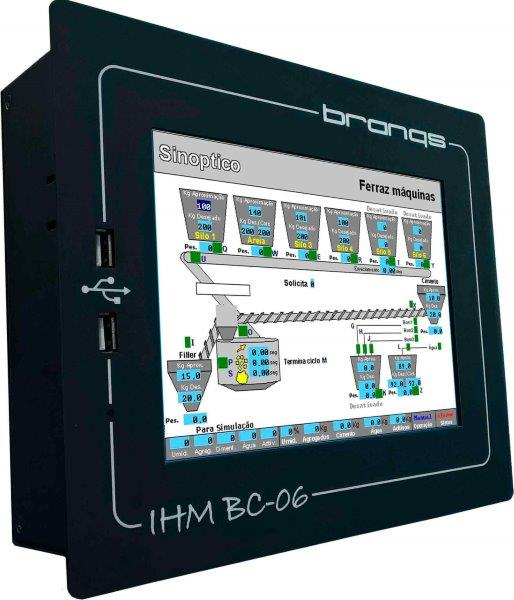
\includegraphics[width=8cm]{figuras/figura-ihm.jpg}}
		}{
			\Fonte{\cite{Branqs}}
		}	
	    \end{figure}
        
    \subsection{Unidade de Aquisição de Dados}
    \label{sec:uad}

        \gls{UAD} são dispositivos que recebem informações relativas ao processo em que estão inseridas e as transferem à um controlador de processo ou diretamente ao sistema de supervisão e controle, onde serão processadas e organizadas para exibição  \cite{mamede-instalacoes}. Dividem-se em duas categorias mais específicas:
        
        \begin{alineascomponto}
        	\item \gls{UD}
        	\item \gls{UADC}
        \end{alineascomponto}
        
    \subsubsection{Unidade Dedicada}
    \label{sec:ud}

    É um dispositivo inserido dentro do processo em que se mantenha apenas uma função dedicada  \cite{mamede-instalacoes}, como exemplos: relés digitais, intertravamento, etc.

    \subsubsection{Unidade de Aquisição de Dados e Controle}
    \label{sec:uadc}

        Tem a função de adquirir dados e controlar ações nos equipamentos respectivos, são compostos por cartões de eletrônicos associados cada um à uma função específica, unidades lógicas, memórias,  entradas e saídas de dados digitais ou analógicos \cite{mamede-instalacoes}.
        
    \subsubsubsection{Unidade Terminal Remota}
    \label{sec:utr}

       \gls{UTR} é uma \gls{UADC} responsável por coletar informações e executar comandos de equipamentos do processo, sejam eles digitais ou analógicos. Possuem capacidade de executar programas em modo local independente do sistema de supervisão, ao mesmo tempo que possui capacidade de integração com o mesmo. Os comandos locais para equipamentos são feitos através de relés de maneira similar ao que ocorre no \gls{CLP}, por rotinas específicas armazenadas em programas gravados na própria \gls{UTR} \cite{mamede-instalacoes}. A Figura \ref{fig:figura-utr} mostra um \gls{UTR} da fabricante WEG, de modelo RUW-03 que possui todas as características aqui descritas.
       
        \begin{figure}[!h]
		\Caption{\label{fig:figura-utr} Exemplo de UTR de modelo RUW-03 da fabricante WEG.}
		%\centering
		\UFCfig{}{
			\fbox{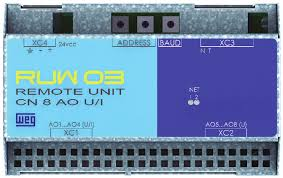
\includegraphics[width=10cm]{figuras/utr-weg.jpg}}
		}{
			\Fonte{\cite{RUW03}}
		}	
	    \end{figure}
       
    \subsubsubsection{Controlador Lógico Programável}
    \label{sec:clp}

       \gls{CLP} é uma \gls{UADC} para controle de equipamentos através de programas desenvolvidos externamente pelo utilizador e nele gravados, simulando à nível de \textit{software} e substituindo: chaves, contatores, temporizadores, relés e outros dispositivos. Permitem a inclusão de cartões eletrônicos para a realização de diferentes tarefas específicas. Possui \gls{IHM}, onde o utilizador pode alterar a programação ou executar tarefas configuradas no \gls{CLP} \cite{mamede-instalacoes}. A Figura \ref{fig:figura-clp} mostra um \gls{CLP} da fabricante WEG, de modelo PLC300 que possui todas as características aqui descritas.
       
        \begin{figure}[!h]
		\Caption{\label{fig:figura-clp} Exemplo de \gls{CLP} de modelo PLC300 da fabricante WEG.}
		%\centering
		\UFCfig{}{
			\fbox{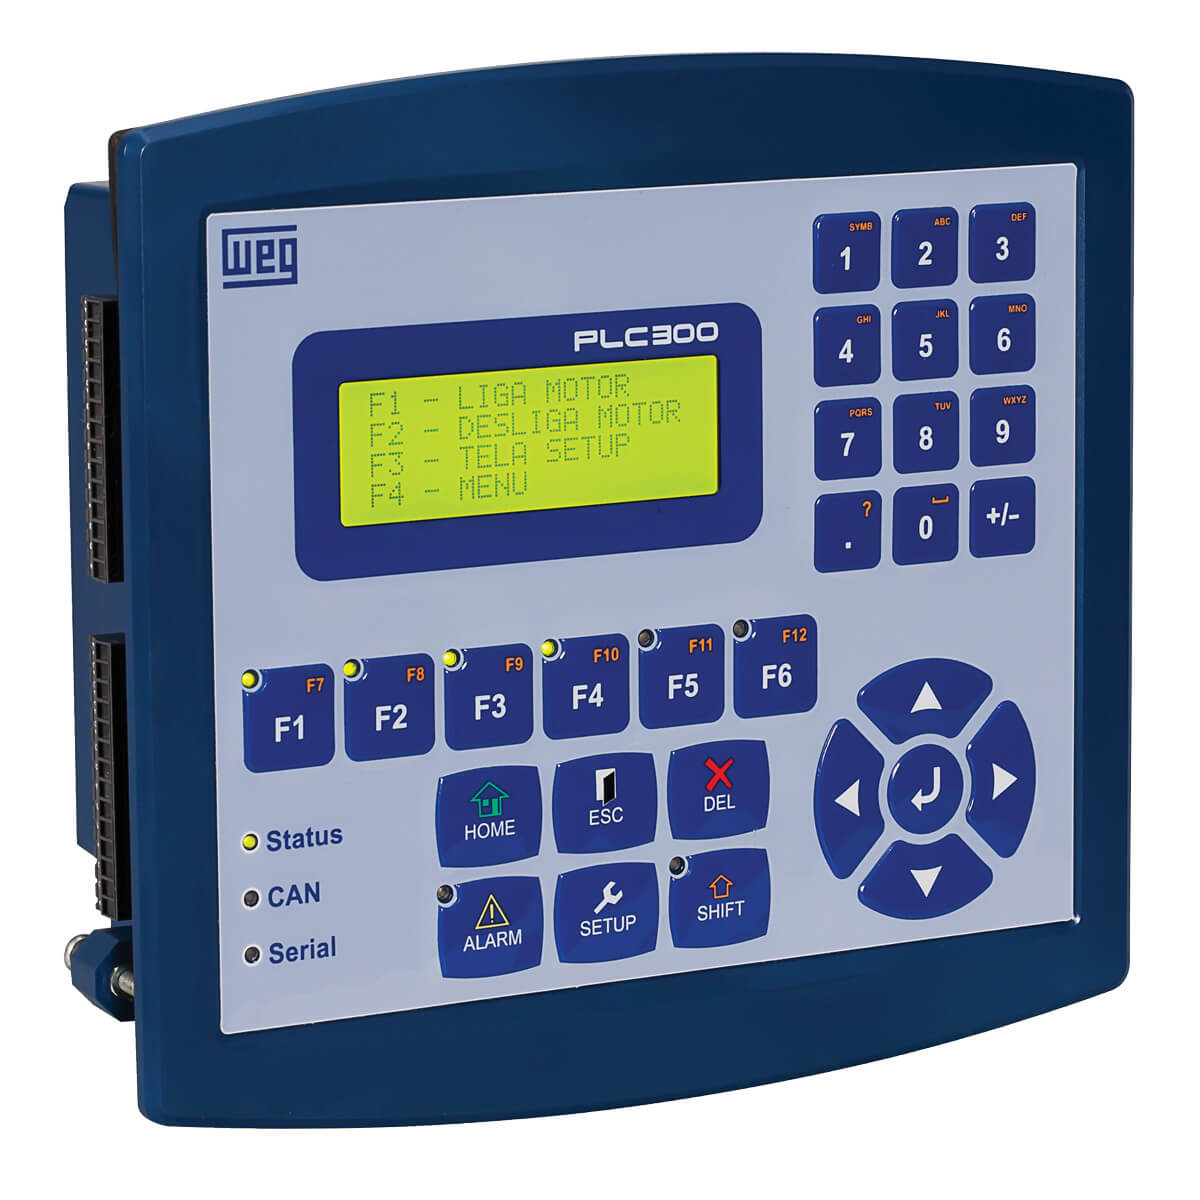
\includegraphics[width=8cm]{figuras/clp-weg.jpg}}
		}{
			\Fonte{\cite{PLC300}.}
		}	
	    \end{figure}

    \section{Protocolos de Comunicação}
    \label{sec:protocolos}
    
    \subsection{Modbus}
    \label{sec:modbus}
    
    Modbus é um protocolo de comunicação de dados voltado à automação industrial. Desenvolvido em 1979, pela \textit{Modicon}, é até hoje utilizado vastamente na indústria em \glspl{CLP} para comandos e aquisição de informações. Podem ser utilizados os padrões: RS-232, RS-485 ou Ethernet para a camada física de ligação, através de sinais discretos ou analógicos. É geralmente utilizado no tipo mestre-escravo, onde os escravos só enviam comunicação quando solicitadas pelo mestre  \cite{Modbus}.
    
    \subsubsection{Modbus Serial}
    \label{sec:modbus-serial}

        Em redes baseadas em RS-232 e RS-485, a comunicação do Modbus é feita de forma serial através de dois modos distintos: \gls{RTU} e \gls{ASCII}. A Figura \ref{fig:figura-modbus-serial} e Tabela \ref{tab:tabela-modbus-serial} representam os pinos da estrutura física RS-485 utilizado pelo Modbus Serial \cite{Modbus}.
        
        No \gls{RTU}, para cada byte transmitido, são codificados 2 caracteres. Os números variam entre -32768 e 32767, o tamanho da palavra RTU é de 8 bits.
        
        \begin{table}[h!]	
        	\centering
        	\Caption{\label{tab:tabela-modbus-rtu} Representação do pacote no modo RTU.}	
        	\IBGEtab{}{
        		\begin{tabular}{crrrr}
        			\toprule
        			Endereço Escravo & Código Função & Dados & CRC \\
        			\midrule \midrule
        			1 byte & 1 byte & 0 a 252 bytes & 2 bytes (CRC-16) \\
        			\bottomrule
        		\end{tabular}
        	}{
        	\Fonte{\cite{Modbus}.}
        }
        \end{table}
        
        No \gls{ASCII}, os dados são codificados com base na tabela \gls{ASCII}, em que cada byte é transmitido através de dois caracteres. O tamanho da palavra ASCII é de 7 bits, utilizando-se caracteres de intervalos 0-9 ou A-F e entre duas mensagens, 3-5 caracteres.
        
        \begin{table}[h!]	
        	\centering
        	\Caption{\label{tab:tabela-modbus-ascii} Representação do pacote no modo ASCII.}	
        	\IBGEtab{}{
        		\begin{tabular}{crrrr}
        			\toprule
        			Início & Endereço & Função & Dados & LRC & Final \\
        			\midrule \midrule
        			":" (ASCII 0x3Ah) & 2 caracteres & 2 caracteres & 0 a 2 x 252 caracteres & 2 caracteres & CR+LF (ASCII 0x0Dh + 0x0Ah) \\
        			\bottomrule
        		\end{tabular}
        	}{
        	\Fonte{\cite{Modbus}.}
        }
        \end{table}
        
        \begin{figure}[!h]
		\Caption{\label{fig:figura-modbus-serial} Pinagem do conector RS485 utilizado no protocolo Modbus Serial.}
		%\centering
		\UFCfig{}{
			\fbox{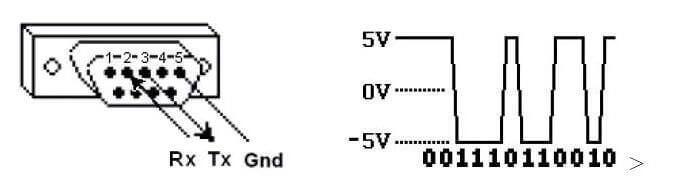
\includegraphics[width=10cm]{figuras/modbus.jpg}}
		}{
			\Fonte{se.com - Acessado em: 28/03/2019}
		}	
	    \end{figure}
	    
	   \begin{table}[h!]	
        	\centering
        	\Caption{\label{tab:tabela-modbus-serial} Pinagem do conector RS485 utilizado no protocolo Modbus Serial.}	
        	\IBGEtab{}{
        		\begin{tabular}{crrrrrr}
        			\toprule
        			Pino &&&&& Sinal \\
        			\midrule \midrule
        			1 &&&&& Não conectado \\
        			2 &&&&& RX - Recepção \\
        			3 &&&&& TX - Envio \\
        			4 &&&&& Não conectado \\
        			5 &&&&& Gnd - Terra \\
        			6 &&&&& Não conectado \\
        			7 &&&&& Não conectado \\
        			8 &&&&& Não conectado \\
        			9 &&&&& Não conectado \\
        			\bottomrule
        		\end{tabular}
        	}{
        	\Fonte{Adaptado de se.com - Acessado em: 28/03/2019}
        }
        \end{table}
        
    \subsubsection{Modbus TCP/IP}
    \label{sec:modbus-tcp}

        As redes baseadas em Ethernet, sob o protocolo \gls{TCP/IP}, se tornaram o método de transporte comum na Internet. O \gls{TCP/IP} é um conjunto de protocolos em camadas, que oferece confiabilidade no transporte de dados entre máquinas, e devido à isso, este padrão torna-se uma opção ideal para sistemas empresariais corporativos. O Modbus \gls{TCP/IP} tornou-se muito utilizado devido sua simplicidade e baixo custo, demandando \textit{hardwares} mínimos para ser utilizado. A maioria dos dispositivos Modbus atualmente presentes no mercado, suportam o padrão \gls{TCP/IP}, aumentando a cada ano a disponibilidade. Há também a possibilidade de conversão entre TCP/IP <=> Serial, onde é possível garantir a retrocompatibilidade entre dispositivos. A Figura \ref{fig:figura-modbus-ethernet} e Tabela \ref{tab:tabela-modbus-ethernet} trazem a representação do conector utilizado no Modbus \gls{TCP/IP} \cite{Modbus}.

        
        \begin{figure}[!h]
		\Caption{\label{fig:figura-modbus-ethernet} Pinagem do conector RJ45 utilizado no protocolo Modbus Ethernet.}
		%\centering
		\UFCfig{}{
			\fbox{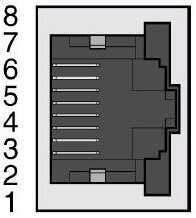
\includegraphics[width=5cm]{figuras/modbus-ethernet.jpg}}
		}{
			\Fonte{Adaptado de se.com - Acessado em: 28/03/2019}
		}	
	    \end{figure}
	    
        \begin{table}[h!]	
        	\centering
        	\Caption{\label{tab:tabela-modbus-ethernet} Pinagem do conector RJ45 utilizado no protocolo Modbus Ethernet.}	
        	\IBGEtab{}{
        		\begin{tabular}{crrrrrr}
        			\toprule
        			Pino &&&&& Sinal \\
        			\midrule \midrule
        			1 &&&&& CAN\_H \\
        			2 &&&&& CAN\_L \\
        			3 &&&&& CAN\_GND \\
        			4 &&&&& D1 - RS485 (Modbus) \\
        			5 &&&&& D0 - RS485 (Modbus) \\
        			6 &&&&& Não conectado \\
        			7 &&&&& VP - Reservado ao conversor RS232/RS485 \\
        			8 &&&&& Comum \\
        			\bottomrule
        		\end{tabular}
        	}{
        	\Fonte{Adaptado de se.com - Acessado em: 28/03/2019}
        }
        \end{table}

        
    \subsection{OPC}
    \label{sec:opc}
    
        \gls{OPC}, inicialmente chamado \textit{Object Linking and Embedding for Process Control}, desenvolvido pela \textit{OPC Foundation} em 1996 e gerenciado por esta desde então, é o padrão de interoperabilidade para o transporte seguro e confiável de informações no espaço industrial, ele é independente de plataforma e garante o fluxo contínuo de informações entre dispositivos de vários fornecedores. É uma série de especificações desenvolvidas por fornecedores do setor, usuários e desenvolvedores. Essas especificações definem a interface entre Clientes e Servidores, bem como Servidores e Servidores, incluindo acesso a dados em tempo real, monitoramento de alarmes e eventos, acesso a dados históricos e outros aplicativos. \cite{OPC}
        
        Seu propósito inicial era agregar vários outros tipos de protocolos distintos de \glspl{CLP}, proprietários ou não, como: Modbus (seção \ref{sec:modbus}), Profibus, etc, de forma simplificada, permitindo que \glspl{IHM} ou \glspl{SCADA} pudessem solicitar informações através de comunicação genérica, permitindo então, que os usuários pudessem implementar sistemas usando os melhores produtos, interagindo perfeitamente via \gls{OPC}.

    \subsubsection{OPC Classic}
    \label{sec:opc-classic}

        Inicialmente, o padrão \gls{OPC} era restrito e baseado na plataforma \textit{Windows}, utilizando \gls{COM/DCOM} para a comunicação entre \textit{softwares}. Como visto na sigla original do \gls{OPC}, ele era suportado por \gls{OLE} voltado à Controle de Processo, essas especificações, agora conhecidas como \gls{OPC} \textit{Classic}, tiveram ampla adoção em vários setores \cite{OPCClassic}. Na Figura \ref{fig:figura-opc-classic} é representado funcionamento de um sistema que utilize \gls{OPC} \textit{Classic}, onde o Servidor \gls{OPC} recebe informações de inúmeros módulos de aquisição de dados, de diferentes fabricantes e diferentes protocolos e permite a interoperabilidade deles com o Cliente \gls{OPC}, de forma genérica.
                
        \begin{figure}[!h]
		\Caption{\label{fig:figura-opc-classic} Diagrama do funcionamento de um sistema que utilize OPC Classic.}
		%\centering
		\UFCfig{}{
			\fbox{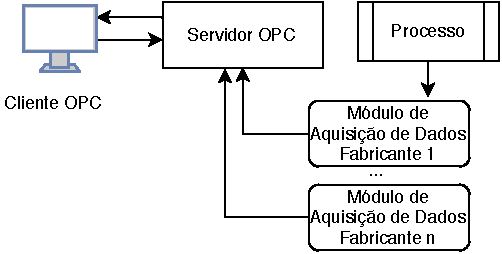
\includegraphics[width=12cm]{figuras/opc.pdf}}
		}{
			\Fonte{O autor}
		}	
	    \end{figure}
	    
	    Existem três definições principais:
        
        \begin{alineascomponto}
        	\item Acesso a Dados - \textit{\gls{OPC} Data Access (DA)}: troca de dados, incluindo valores, tempo e informações de qualidade.
        	\item Alarmes e Eventos - \textit{\gls{OPC} Alarms \& Events (AE)}: troca de mensagens de alarmes e tipos de eventos, estados de variáveis e gerenciamento de estados.
        	\item Acesso a Dados Históricos - \textit{\gls{OPC} Historical Data Access (HDA)}: define os métodos de consulta e quais análises podem ser aplicadas a dados históricos, com registro de data e hora.
        \end{alineascomponto}

    \subsubsection{OPC-UA}
    \label{sec:opc-ua}

        Com a introdução de arquiteturas orientadas a serviços em sistemas de manufatura, surgiram novos desafios em segurança e modelagem de dados, a \textit{OPC Foundation} desenvolveu as especificações do \gls{OPC-UA} em 2008, sendo uma arquitetura orientada a serviços independentes, aberta e escalável.
        
	    \begin{figure}[!h]
		\Caption{\label{fig:figura-opc-ua} Diagrama do funcionamento de um sistema que utilize OPC-UA.}
		%\centering
		\UFCfig{}{
			\fbox{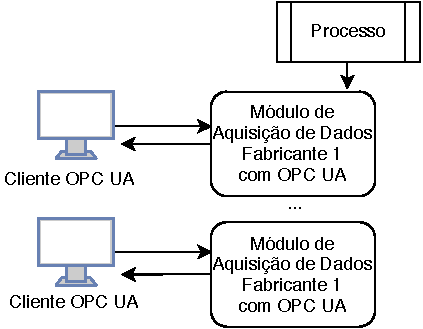
\includegraphics[width=10cm]{figuras/opc-ua.pdf}}
		}{
			\Fonte{O autor}
		}	
	    \end{figure}
        
        O \gls{OPC-UA} integra todas as funcionalidades do \gls{OPC} \textit{Classic}, além de outras melhorias, como:
        
        \begin{alineascomponto}
        	\item Segurança: criptografia de 128 ou 256 bits, verificação de erros para que a mensagem recebida seja exatamente a mensagem enviada, autenticação através de certificados e níveis de permissão.
        	\item Extensível: é possível adicionar novos recursos mantendo a compatibilidade com aplicações já existentes.
        	\item Descoberta: permite a busca por servidores \gls{OPC} na rede ou em computadores.
        	\item Hierarquia: todos os dados são dispostos de forma hierárquica, permitindo informações simples e complexas na mesma estrutura.
        	\item Auditoria: os dados à serem lidos/escritos possuem permissões de acesso tais como registros sobre sua utilização.
        	\item Independência de plataforma: funciona em computadores tradicionais e servidores em nuvem, seja o sistema operacional \textit{Linux}, \textit{Windows} ou outros, \glspl{CLP}, micro-controladores, etc.
        	
        \end{alineascomponto}
	    
    \subsection{HTTP}
    \label{sec:http}
    \gls{HTTP}, coordenado pela \gls{W3C}, é um protocolo de comunicação à nível de aplicação para distribuição de informação de hipermídia, é base para comunicação pela \gls{WEB} desde 1990. Inicialmente, em sua versão HTTP/0.9, era um simples protocolo de transferência de dados não tratados através da Internet e em sua versão atual HTTP/1.1, lançado em 1999, foram implementadas outras funcionalidades como a possibilidade de troca de mensagens no formato \gls{MIME}, que carregam consigo metainformações sobre a requisição ou resposta e o corpo das informações transferidas \cite{HTTP}.
    
    A transferência de informação acontece através de \textit{sockets} sob o protocolo \gls{TCP/IP}, onde com a arquitetura cliente-servidor, o cliente envia uma requisição ao servidor, com o padrão \gls{MIME} e  localizado através endereços, como o \gls{URI}, que identifica a informação acessada e \gls{URL}, que determina a localização desta informação, a conexão é completada e o servidor retorna o \textit{status} de acordo com o sucesso ou não da requisição e possíveis conteúdos também em formato \gls{MIME} caso sejam necessários, encerrando assim a conexão.
    
        \subsubsection{HTTPS}
        \label{sec:https}
        O \gls{HTTPS} é uma derivação do protocolo de comunicação \gls{HTTP} para mensagens seguras, projetado como uma camada de segurança utilizando o protocolo \gls{TLS}. Além de fornecer uma variedade de mecanismos de segurança para clientes e servidores, não são necessárias chaves públicas do lado cliente, suporta criptografia ponta a ponta e torna possível verificar a autenticidade do servidor através de certificados digitais. Seu uso é recomendado em redes inseguras, evitando a clonagem das informações trafegadas que poderia acontecer na ausência de criptografia \cite{HTTPS}. Segundo \cite{usoHTTPS}, em fevereiro de 2019, mais de 58.44\% dos 1 milhões \textit{websites} mais visitados da \textit{internet} já utilizavam o \gls{HTTPS}.
        
        \subsubsection{REST}
        \label{sec:rest}

        O \gls{REST} é um estilo de arquitetura para \textit{\gls{WEB} Service},  uma solução padronizada pela \gls{W3C} e \gls{OASIS} que busca fornecer interoperabilidade entre dispositivos e aplicações pela internet utilizando diferentes tipos de linguagens, o que a torna compatível com a maioria das aplicações já existentes \cite{W3C}.
        
        O envio e recebimento das mensagens é realizada de forma simplificada através dos protocolos \gls{HTTP} ou \gls{HTTPS} utilizando os formatos: \gls{XML}, \gls{JSON} ou \gls{HTML} e métodos de chamada bem definidos: GET, POST, PUT, PATCH e DELETE. Comumente utilizado por empresas no o desenvolvimento de \gls{API} para acesso a informações específicas sobre serviços, aplicações, faturas, etc. A Figura \ref{fig:figura-mqtt1} traz uma ideia geral sobre o funcionamento de uma API que utiliza a arquitetura REST para troca dos dados.
            
            \begin{figure}[!h]
    		\Caption{\label{fig:figura-rest1} Representação do funcionamento de uma API REST.}
    		%\centering
    		\UFCfig{}{
    			\fbox{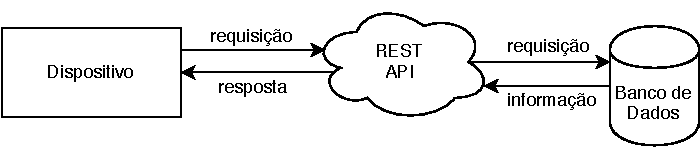
\includegraphics[width=15cm]{figuras/figura-rest1.pdf}}
    		}{
    			\Fonte{O autor}
    		}	
    	    \end{figure}
    	
    	\subsubsection{Métodos de Chamada}
    	\label{sec:metodos-chamada}
    	
    	Quando uma nova requisição é feita, é necessário definir o método que será utilizado. Os métodos de chamada são padronizados para o protocolo \gls{HTTP} e são conhecidos como verbos, pois identificam a ação que será executada pela requisição. Os mais comuns são:
    	
        \begin{alineascomponto}
        	\item GET: Apenas recebe informações, as requisições devem ser seguras e idempotentes, ou seja, independente de quantas vezes ela seja repetida, com os mesmos parâmetros, o resultado sempre deve ser o mesmo. Podem haver solicitações parciais ou condicionais.

            \item POST: Envia e recebe de informações, é utilizado na criação de novos "objetos"  (elementos da aplicação), mas também é comum o uso para atualização destes.
            
            \item PUT: Envia e recebe de informações, é utilizado na atualização de "objetos" já existentes, na falta do envio de algumas informações necessárias, estas são considerados nulas ou vazias. Assim como o GET, o PUT é idempotente.
            
            \item PATCH: Envia e recebe de informações, similar ao PUT,  é utilizado na atualização de "objetos" já existentes, porém, apenas os campos especificados.

            \item DELETE: Envia e recebe de informações, é utilizado na exclusão de "objetos", podendo ser imediato ou não.
        \end{alineascomponto}
        
        \begin{table}[h!]	
        	\centering
        	\Caption{\label{tab:tabela-modbus-ethernet} Comparativo entre os métodos de chamada.}	
        	\IBGEtab{}{
        		\begin{tabular}{crrrr}
        			\toprule
        			Método & Descrição & Seguro & Idempotente \\
        			\midrule \midrule
        			GET & Recebe informações & sim & sim \\
        			POST & Cria objetos & não & não \\
        			PUT & Atualiza objetos, na falta de informações, considera como nulas & não & sim \\
        			PATCH & Atualiza objetos, alterando apenas as informações enviadas & não & não \\
        			DELETE & Exclui objetos, imediatamente ou não & não & sim \\
        			\bottomrule
        		\end{tabular}
        	}{
        	\Fonte{O autor}
        }
        \end{table}

    	\subsubsection{Formatos de Conteúdo}
    	\label{sec:formatos-de-conteudo}
    	São tipos de linguagem de marcação para necessidades especiais com a finalidade de transferência de informações pela \textit{internet}. Os mais comuns são:
    	
        \begin{alineascomponto}
        	\item \gls{HTML} (texto puro).
            \item \gls{XML}:  É baseado em texto simples, de simples leitura, pode representar listas, registros e árvores. Seu próprio formato descreve sua estrutura, campos e valores, os dados são organizados de forma hierárquica e é editável em qualquer ambiente \cite{XML}. A Figura \ref{fig:figura-xml} traz um exemplo de utilização do formato \gls{XML}.
                \begin{figure}[!h]
        		\Caption{\label{fig:figura-xml} Exemplo de informações organizadas no formato XML.}
        		%\centering
        		\UFCfig{}{
        			\fbox{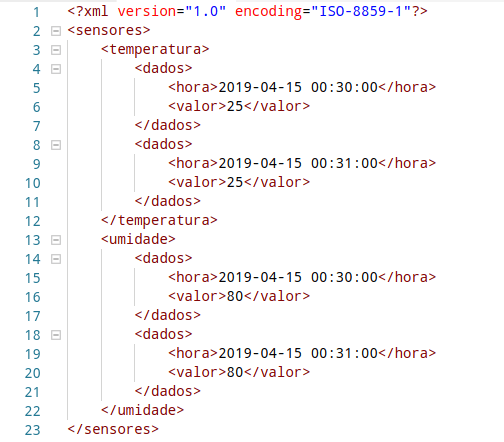
\includegraphics[width=10cm]{figuras/exemploXML.png}}
        		}{
        			\Fonte{O autor}
        		}	
        	    \end{figure}
            \item \gls{JSON}: É um formato leve de informações, de simples leitura e análise. Assim como o \gls{xml} é hierárquico, em pares, ou seja, para cada rótulo, há um valor associado ou sub-conjunto destes. A Figura \ref{fig:figura-json} traz um exemplo de utilização do formato \gls{JSON} \cite{JSON}.
                \begin{figure}[!h]
        		\Caption{\label{fig:figura-json} Exemplo de informações organizadas no formato JSON.}
        		%\centering
        		\UFCfig{}{
        			\fbox{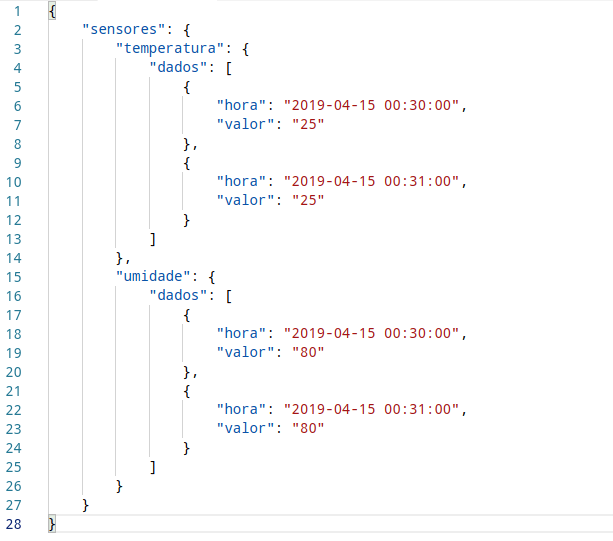
\includegraphics[width=11cm]{figuras/exemploJSON.png}}
        		}{
        			\Fonte{O autor}
        		}	
        	    \end{figure}
        \end{alineascomponto}

    \subsection{MQTT}
    \label{sec:mqtt}

        O \gls{MQTT} foi desenvolvido por Dr. Andy Stanford-Clark, da IBM, e Arlen Nipper, da Arcom no ano de 1999. É um protocolo de mensagens extremamente simples e leve, projetado para ser utilizado em dispositivos que tenham restrição de largura de banda, alta latência ou baixa confiabilidade. Baseia-se na topologia publicador/assinatura, onde as mensagens são enviadas com identificação através de tópicos (\textit{topics}) ou sub-tópicos, o que permite uma única mensagem ser destinada à múltiplos receptores com apenas um envio, ou da mesma forma, receber informações agrupadas de vários sub-tópicos. O elemento responsável pelo envio e recebimento de mensagens é denominado \textit{broker}, que funciona como uma central, intermediando as informações enviadas pelos dispositivos e aplicações da rede \cite{MQTT}. A Figura \ref{fig:figura-mqtt1} apresenta um exemplo de utilização ao qual um subscritor (possível dispositivo associado à rede) recebe informações de dois sensores utilizando um único tópico.
        
        \begin{figure}[!h]
		\Caption{\label{fig:figura-mqtt1} Representação do funcionamento do MQTT.}
		%\centering
		\UFCfig{}{
			\fbox{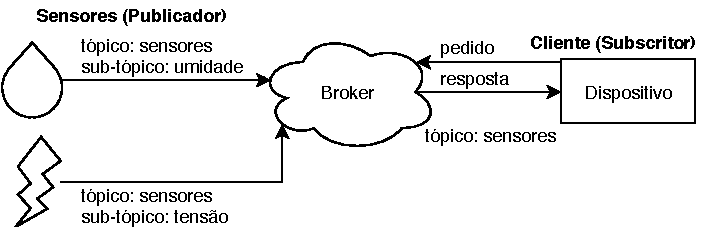
\includegraphics[width=15cm]{figuras/figura-mqtt1.pdf}}
		}{
			\Fonte{O autor}
		}	
	    \end{figure}
	    
	    A autenticação é feita através de usuário e senha, com a possibilidade de conexão criptografada e a escolha de três níveis de serviço (prioridades na transmissão) que dependerá do projeto em questão, qualidade de conexão do dispositivo, entre outros, sendo elas: 
	    
        \begin{alineascomponto}
        	\item Nível 0: Não é feita quaisquer confirmações sobre a entrega da informação, de forma que a mensagem é descartada após o envio.
        	\item Nível 1: São feitas várias tentativas de entrega até que se obtenha confirmação no recebimento, mesmo que isso implique no recebimento em duplicidade.
        	\item Nível 2: Há garantia de que a mensagem só será entregue uma vez, havendo tanto a confirmação de entrega da mensagem como a confirmação da confirmação de entrega.
        \end{alineascomponto}
        
    \section{SCADA}
    \label{sec:scada}

        Sistemas de Supervisão e Aquisição de Dados, do inglês, \gls{SCADA}, consistem basicamente de \textit{softwares} que monitoram e operam partes de um ou mais processos, através de comunicação específica por módulos de aquisição de dados ou com controladores de processos, como o \gls{CLP}, que por sua vez, são conectados fisicamente ao servidor de dados ou através de rede. Com o domínio sobre as informações do processo, esta ferramenta é capaz de apresentar através de uma \gls{IHM} e de forma simplificada, valores e estados gerais do processo que se deseja atuar, desta forma, obtêm-se um maior controle sobre a tarefa, pois é possível centralizar a leitura de todos os sensores atuantes, a categorização e histórico destes dados, além da priorização de pendências do processo, reduzindo assim a necessidade um maior número de trabalhadores especializados que desempenhem a mesma função. \cite{WhatScada}
        
        O \gls{SCADA} apresenta uma série de vantagens, dentre elas: (i) redução de custos, devido a possibilidade de geração de relatórios detalhados úteis ao planejamento estratégico, evidenciando possíveis vícios do processo produtivo, (ii) maior desempenho na produção, por determinar os valores ótimos de trabalho, (iii) confiabilidade e continuidade, devido a existência de alarmes críticos, ou seja, notificações visuais ao operador, quando alguma variável ou condição do processo esteja em desacordo com o padrão de operação, desta forma, possíveis problemas que ocasionariam uma maior parada na produção, são mitigados com intervenções de forma quase imediata pelo operador caso sejam necessárias, trazendo assim vantagem competitiva. XX
        
        Todas as informações do processo podem coletadas e armazenadas em tempo real em um banco de dados, podendo serem implementadas no sistema de gestão empresarial da empresa ou utilizadas para cálculos mais complexos, sendo o último realizado por outras máquinas para garantir a que o \gls{SCADA} não tenha seu desempenho prejudicado.
        Uma representação básica do sistema \gls{SCADA} é ilustrada na Figura \ref{fig:figura-scada1}, ao qual todas as informações do processo são centralizadas e exibidas de forma simplificada ao colaborador. 
        
        \begin{figure}[!h]
		\Caption{\label{fig:figura-scada1} Arquitetura física básica \gls{SCADA}.}
		%\centering
		\UFCfig{}{
			\fbox{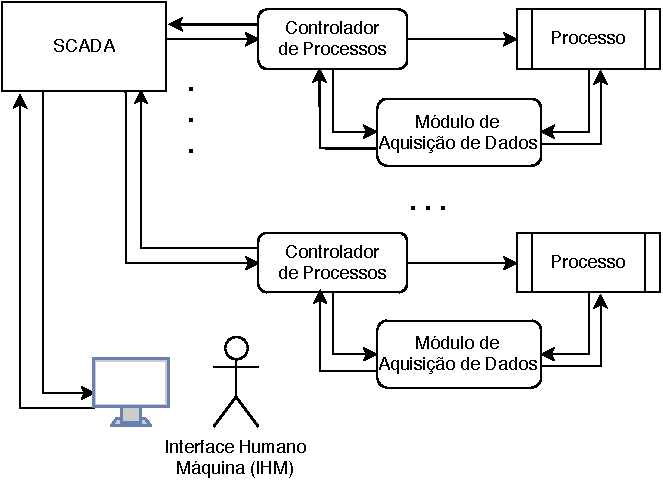
\includegraphics[width=14cm]{figuras/figura-scada1.pdf}}
		}{
			\Fonte{O autor}
		}	
	    \end{figure}
	    
    \subsection{SCADA WEB}
    \label{sec:scadaweb}
    
    \gls{WEB}, ou Rede Mundial de Computadores, é como se designa o sistema de hiperligações e marcação de texto que permitem a disponibilidade de conteúdo através da \textit{internet}, como: páginas de texto, documentos, músicas, entre outros \cite{W3C}. O \gls{SCADA} \gls{WEB} é uma versão elaborada do SCADA convencional, onde os dados são transferidos para servidores na \textit{internet} e posteriormente processados, integrados às demais plataformas e/ou vistos em páginas WEB. A transição do SCADA para \gls{SCADA} \gls{WEB} ocorre principalmente devido à superação de uma baixa largura de banda e restrições de comunicação como ocorria antigamente. Os avanços tecnológicos possibilitaram a rápida expansão dos canais de dados através da \textit{internet}, onde até mesmo a transmissão de informações em tempo real, não é mais um fator limitante. \cite{ScadaWebSimp}
    
    Sistemas \gls{SCADA} com base na \textit{internet} podem se tornar uma parte importante do funcionamento de sistemas de controle, onde o \gls{XML} e outras linguagens disponíveis, podem oferecer possibilidade de resolução de problemas de incompatibilidade que existiam no \gls{SCADA} convencional, onde as fontes de comunicação com o processo são físicas e tornam necessários protocolos de comunicação específicos para qualquer adaptação. Independente de como são obtidas as informações, a visualização deve ser simples ao usuário, onde antes seria feita através de uma \gls{IHM}, este ato se reduz à um simples \textit{smartphone} ou página no navegador, sem ser necessária a instalação de qualquer \textit{software} adicional. A convergência das novas tecnologias, afeta drasticamente a supervisão destas informações, possibilitando controle distribuído e a possibilidade de armazenamento destas informações em qualquer lugar do mundo, com uma ampla capacidade de recursos \cite{ScadaWebInterOp}. Uma representação básica do sistema \gls{SCADA} \gls{WEB} é ilustrada na Figura \ref{fig:figura-scada-web1}, onde as informações de um grupo de plantas são centralizadas e exibidas de forma simplificada ao colaborador.
    
    \begin{figure}[!h]
	\Caption{\label{fig:figura-scada-web1} Arquitetura de um \gls{SCADA} \gls{WEB}.}
	%\centering
	\UFCfig{}{
		\fbox{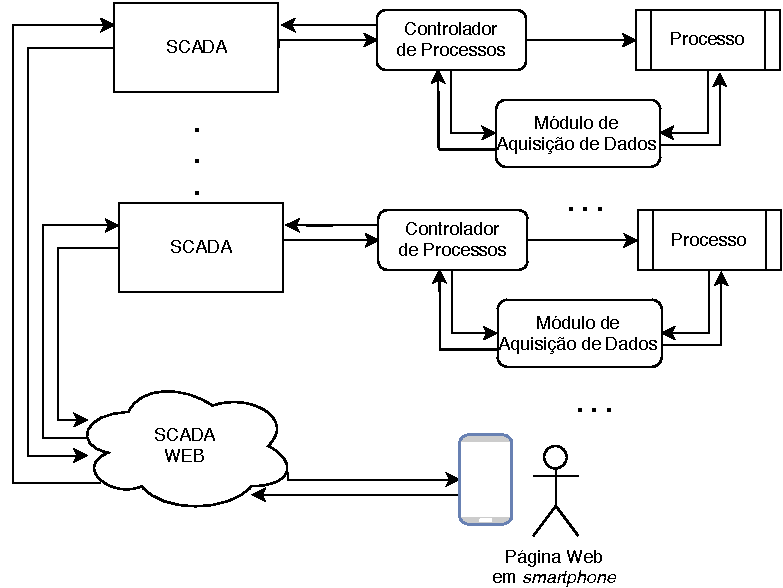
\includegraphics[width=15cm]{figuras/figura-scada-web1.pdf}}
	}{
		\Fonte{O autor}
	}	
    \end{figure}
    
    A implementação de um \gls{SCADA} \gls{WEB}, não só abre possibilidade de armazenamento de dados global, como também eleva a capacidade de recursos computacionais à um nível muito superior, devido à possibilidade de utilização de servidores em nuvem - interligação de vários servidores através da internet formando um núcleo único de processamento - é possível controlar além de grupos de processos, grupos de plantas. Segundo \cite{ScadaNextGer}, a nova geração do \gls{SCADA} pode modificar significamente a forma de projetar e implementar os processos industriais no futuro, onde o sistema terá que lidar com uma quantidade muito superior de dados distribuídos e informações em tempo real para tomar as decisões baseadas neste dados com informações internas e externas. A \gls{IHM} fica não mais limitada à um local físico, mas acessível através de todos os computadores, \textit{smartphones} e \textit{tablets} conectados à \textit{internet}, permitindo a colaboração simultânea na supervisão do processo. Com o uso de várias plantas simultâneamente, há a possibilidade de implementação de uma rotina \gls{QoS}, ou Nível de Serviço, que gerencia prioridades de conexão, dependendo das necessidades dinâmicas de cada planta.
    
    A desvantagem é a robustez do sistema.
    
    \subsection{Sistemas SCADA}
    \label{sec:sistemas-scada}
    
    \subsubsection{Sistemas proprietários}
    \label{sec:sistemas-scada-proprietarios}
    
	\subsubsubsection{Elipse E3}
    \label{sec:elipse}

        O Elipse E3 \cite{Elipse}, desenvolvido pela empresa Elipse Software, representa a terceira geração do \gls{SCADA}. Utiliza o conceito de múltiplas camadas, onde incluem: servidores, regras de aplicação ou de negócio e estações clientes. O sistema é composto por 3 aplicações: 
        
        \begin{alineascomponto}
        	\item \textit{E3Server}: é o servidor das aplicações, em que se gerencia todos os processos de execução do \textit{software} e processa a comunicação entre eles. Suas ações são basicamente: envio das informações gráficas e dados para o cliente, gerenciamentos dos processos de E/S e comunicação com os diversos pontos de aquisição, controle da cópia de produtos, cliente e servidor OPC e sincronismo de alarmes e bases de dados. Permite também a distribuição deste serviço entre várias máquinas de acordo com a necessidade, com objetivo de manter a continuidade em uma eventual falha.
        	\item \textit{E3Viewer}: responsável pela interface de operação e visualização da aplicação que se encontra no E3Server, com operação local ou via \textit{intranet}/\textit{internet}, pode ser acessado por diversas plataformas como: Mac OS, Linux, Windows CE ou ainda, há a possibilidade de utilização do E3WebServer para gerenciamento adicional do acesso via Internet.
        	\item \textit{E3Studio}: ferramenta para configuração do sistema, servindo como plataforma universal do desenvolvimento. A configuração e execução compartilham da mesma base de dados, de forma que as edições das aplicações podem ser enviadas em \textit{runtime}, sem ser necessário a parada da aplicação, independente de ser feita local ou remotamente. É possível a edição de mais de um aplicativo ao mesmo tempo ou a edição ser feita por mais de uma pessoa devido compartilharem o mesmo servidor. Possui ferramentas, como: editores de telas, relatórios e \textit{scripts}.
        \end{alineascomponto}
        
        \begin{figure}[!h]
		\Caption{\label{fig:figura-elipse-e3} Demonstração da tela de processo do \textit{software} Elipse E3.}
		%\centering
		\UFCfig{}{
			\fbox{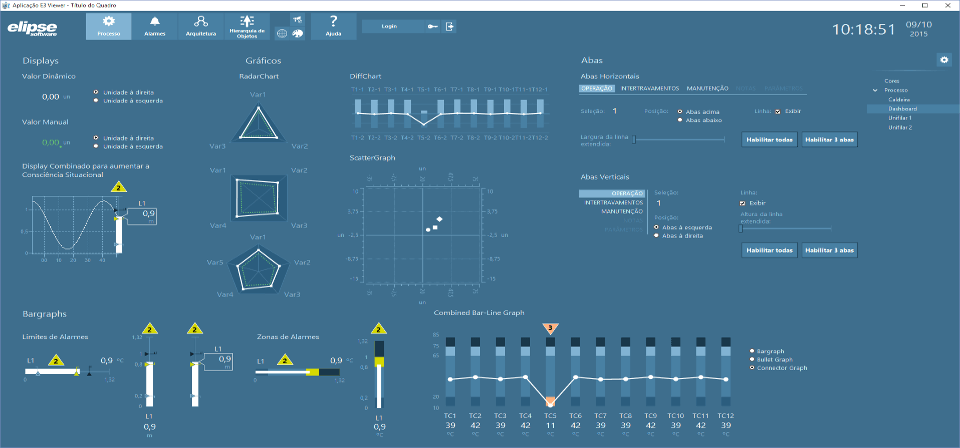
\includegraphics[width=15cm]{figuras/elipse-e3.png}}
		}{
			\Fonte{\cite{Elipse}.}
		}	
	    \end{figure}

	    
	    Outras informações importantes:
	    
	    \begin{alineascomponto}
        	\item Possui drivers para comunicação com mais de 300 tipos de dispositivos e sistemas, sejam eles proprietários ou \gls{OPC}, além de produzir drivers sob encomenda.
        	\item Possui interfaces específicas para Access (.MDB), SQL Server/MSDE, Oracle ou acesso genérico através de padrões ADO e ODBC, faz acesso à base de dados corporativas fazendo o interfaceamento entre o processo e sistemas administrativos, de produção, manutenção e gestão.
        \end{alineascomponto}
	    
	\subsubsubsection{InduSoft Web Studio®}
    \label{sec:indusoft}

        O InduSoft Web Studio® \cite{InduSoft}, desenvolvido pela empresa InduSoft, fornece componentes básicos de automação para o desenvolvimento de \glspl{IHM}, sistemas \glspl{SCADA} e soluções de instrumentação embarcada. O sistema é composto por 2 aplicações:
        
        \begin{alineascomponto}
            \item \textit{Server}: é o servidor das aplicações, em que se gerencia todos os processos de execução do \textit{software} e processa a comunicação entre eles. Suas ações são basicamente: envio das informações gráficas e dados para o cliente, gerenciamentos dos processos de entrada e saída e comunicação com os diversos pontos de aquisição, controle da cópia de produtos, servidor OPC e sincronismo de alarmes e bases de dados.
        	\item \textit{IoTViewer}: responsável pela interface de operação e visualização da aplicação que se encontra no \textit{Server}, com operação local ou via \textit{intranet}/\textit{internet}.
        \end{alineascomponto}
    
        \begin{figure}[!h]
		\Caption{\label{fig:figura-indusoft} Demonstração da tela de processo do \textit{software} InduSoft Web Studio®.}
		%\centering
		\UFCfig{}{
			\fbox{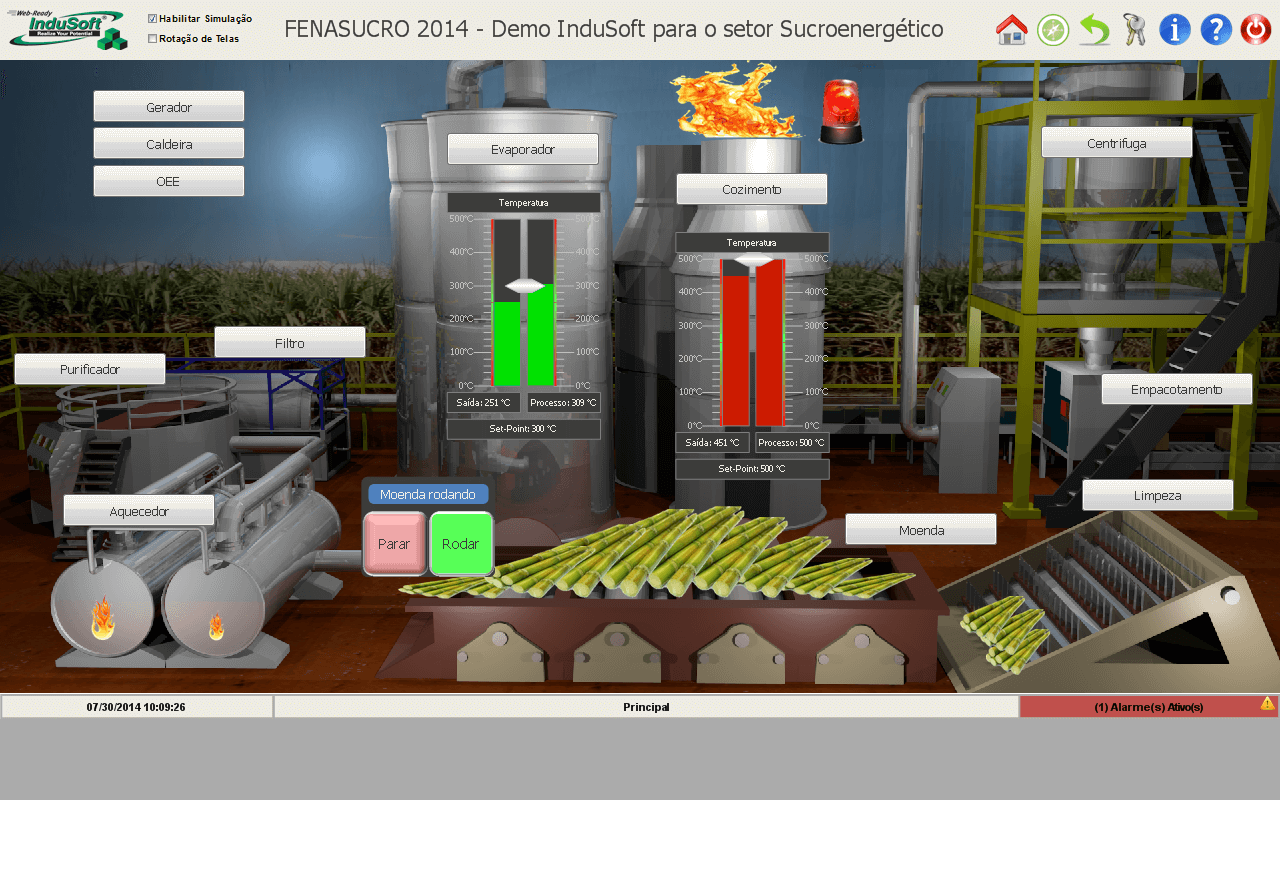
\includegraphics[width=15cm]{figuras/indusoft.png}}
		}{
			\Fonte{\cite{InduSoft}.}
		}	
	    \end{figure}
	    
        Outras informações importantes:
        
        \begin{alineascomponto}
        	\item A aplicação \textit{Server} suporta as plataformas \textit{Microsoft}, como: \textit{Windows CE, Mobile, XP Embedded e Server}, enquanto a aplicação cliente, o \textit{IoTView}, pode também suportar plataformas, como: \textit{Linux e VXWorks}.
        	\item Permite visualização de processo através de Navegador \gls{WEB}, podendo ser acessado através de celulares ou computadores de mesa, seja em rede local ou pela \textit{internet}.
        	\item Possui suporte para \gls{CLP} ou controlador e drivers para comunicação com mais de 200 tipos de dispositivos e sistemas, sejam eles proprietários ou \gls{OPC}, além de comunicação por \gls{TCP/IP}.
        	\item Alarmes podem ser enviados via \textit{e-mail}, celulares ou através do próprio navegador.
        	\item Permite acesso à base de dados corporativas fazendo o interfaceamento entre o processo e sistemas administrativos, de produção, manutenção e gestão.
        \end{alineascomponto}


    \subsubsection{Sistemas de código aberto}
    \label{sec:scadaweb}
    
	\subsubsubsection{ScadaBR}
    \label{sec:scadabr}

        O ScadaBR \cite{ScadaBR} é um \textit{software} livre e de código-fonte aberto. Abrange profissionais de automação, universidades, escolas técnicas e empresas de todos os portes. O projeto foi iniciado em 2006, por iniciativa da empresa MCA Sistemas com sede em Florianópolis - SC, que com o auxílio de outras empresas, a fundação CERTI e a Universidade Federal de Santa Catarina - UFSC, desenvolveram o sistema de forma completa em português baseado no \textit{software} Mango. Possui apoio da FINEP, SEBRAE e CNPq, que também, financiaram a iniciativa durante 2 anos.

        \begin{figure}[!h]
		\Caption{\label{fig:figura-indusoft} Demonstração de telas, incluindo a de processo, do \textit{software} ScadaBR.}
		%\centering
		\UFCfig{}{
			\fbox{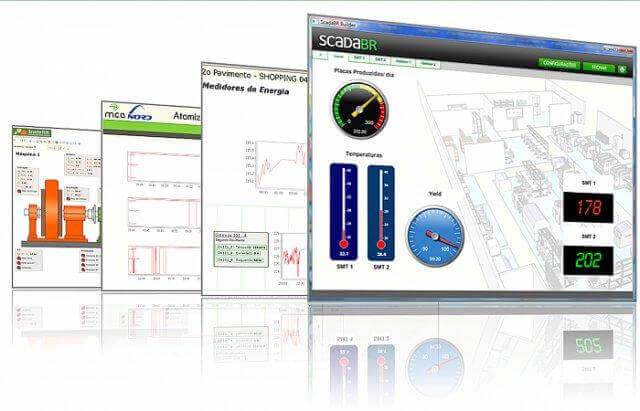
\includegraphics[width=15cm]{figuras/scadabr.jpg}}
		}{
			\Fonte{\cite{ScadaBR}.}
		}	
	    \end{figure}
	    
	    Outras informações importantes:
	    
	    \begin{alineascomponto}
    	    \item A aplicação \textit{Server} suporta diferentes plataformas, como: \textit{Windows} 32/64 bits e \textit{Linux}.
    	    \item Permite visualização de processo através de Navegador \gls{WEB}, podendo ser acessado através de celulares ou computadores de mesa, seja em rede local ou pela \textit{internet}.
        	\item Possui mais de 20 protocolos de comunicação, como: Modbus \gls{TCP/IP} e Serial, \gls{HTTP}, etc.
        	\item Customização de \textit{scripts} para controle, automação, etc.
        	\item Possibilidade de cálculos com funções matemáticas, estatísticas etc, com as variáveis do processo.
        	\item Níveis de permissão de usuários, com controle de acesso.
        \end{alineascomponto}
	    
	\subsubsubsection{TANGO Controls}
    \label{sec:tango}

        O TANGO Controls \cite{Tango} é um \textit{software} livre e de código-fonte aberto. Foi desenvolvido pelo \textit{European Synchrotron Radiation Facility} em Genebra, França e seu desenvolvimento já supera 20 anos de duração. Foi desenvolvido principalmente para necessidades de instalações de pesquisas, com o conceito agregado de ser criado um novo \textit{framework}. Pode ser executado de forma autônoma ou distribuída, local ou remota.

        \begin{figure}[!h]
		\Caption{\label{fig:figura-tango} Demonstração da tela de processo do \textit{software} TANGO Controls.}
		%\centering
		\UFCfig{}{
			\fbox{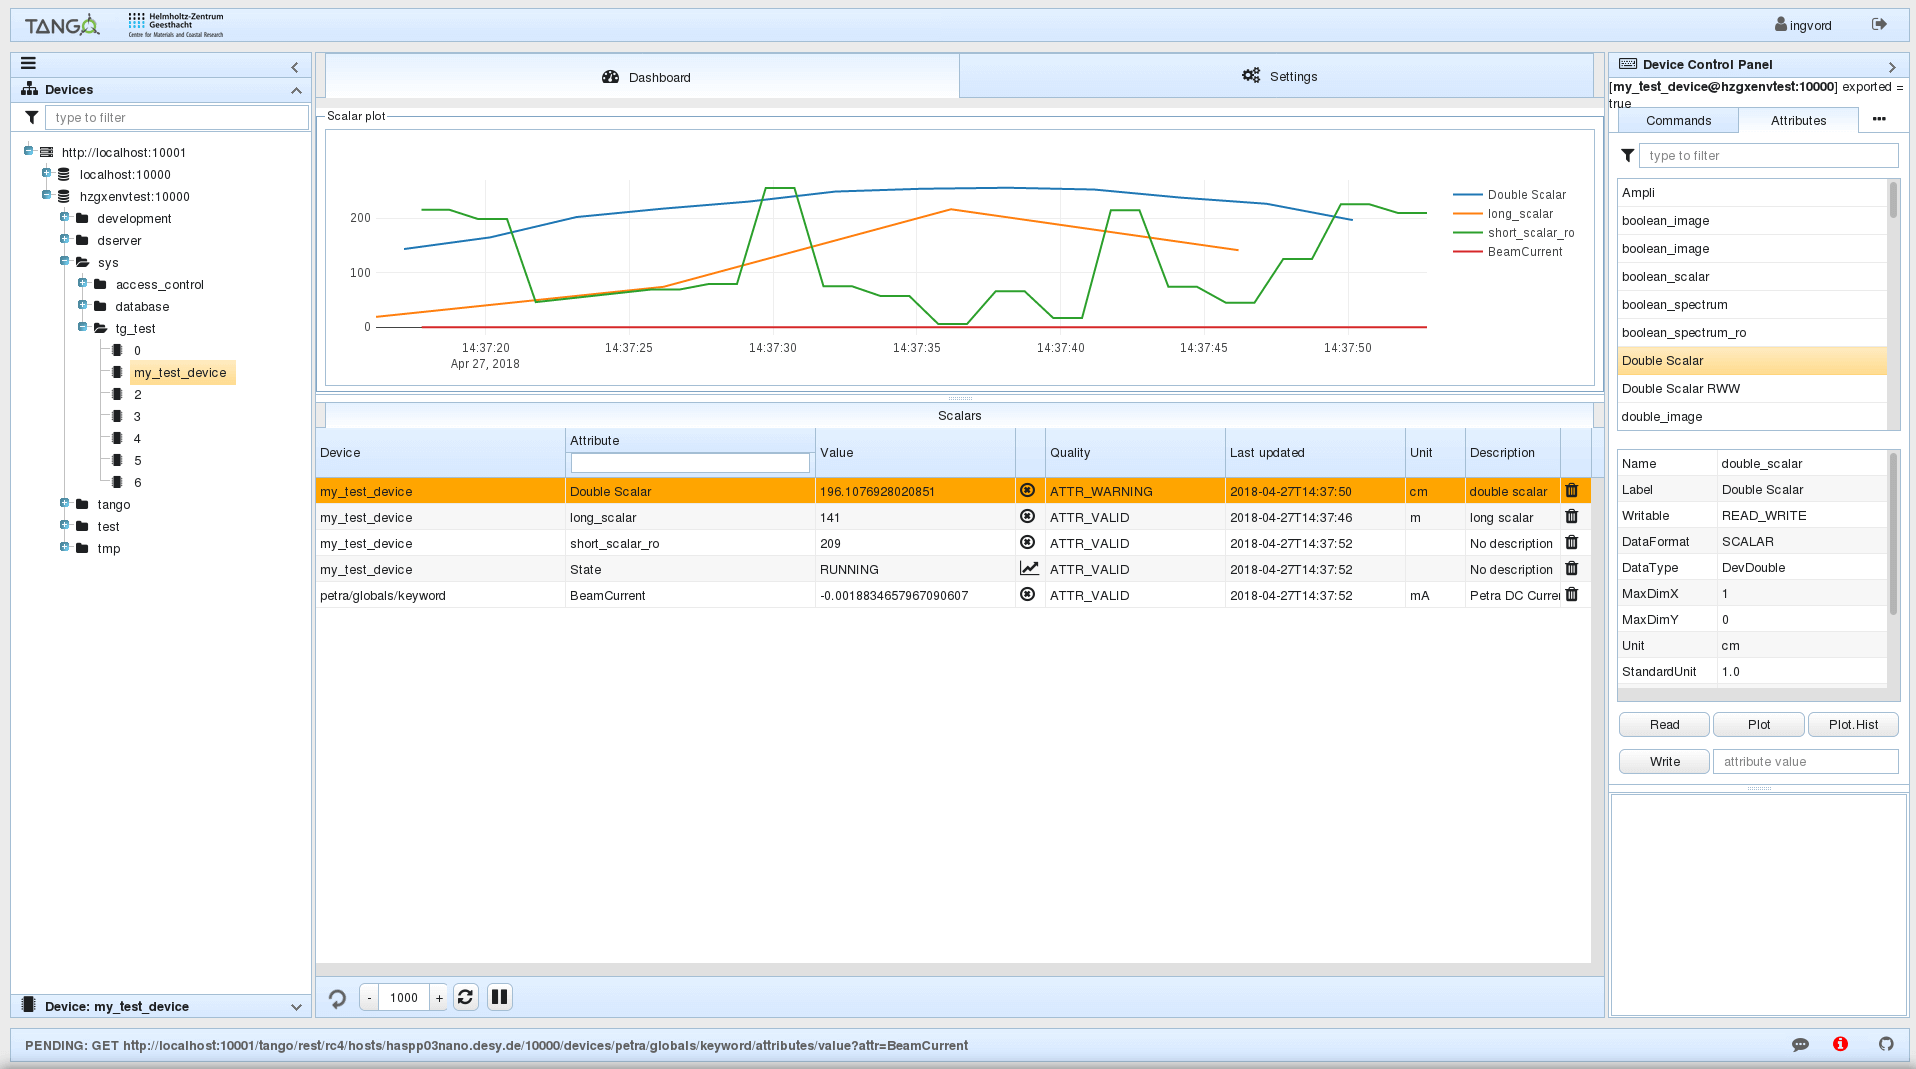
\includegraphics[width=15cm]{figuras/tango.png}}
		}{
			\Fonte{\cite{Tango}.}
		}	
	    \end{figure}
	    
	    Outras informações importantes:
	    
	    \begin{alineascomponto}
    	    \item Permite visualização de processo através de Navegador \gls{WEB}, podendo ser acessado através de celulares ou computadores de mesa, seja em rede local ou pela \textit{internet}.
        	\item Possui diversos \textit{drivers} de comunicação, disponibilizados de forma gratuita.
        	\item Permite a adição de funções analíticas para a tomada de decisões.
        	\item Encontra-se em fase de transição para atender a demanda \textit{IoT} industrial.
        \end{alineascomponto}
	    
	\subsubsubsection{Rapid SCADA}
    \label{sec:rapidscada}

        O Rapid SCADA \cite{RapidSCADA} é um \textit{software} livre e de código-fonte aberto, desenvolvido pela empresa russa \textit{Rapid Software}.

        \begin{figure}[!h]
		\Caption{\label{fig:figura-rapidscada} Demonstração da tela de processo do \textit{software} Rapid SCADA.}
		%\centering
		\UFCfig{}{
			\fbox{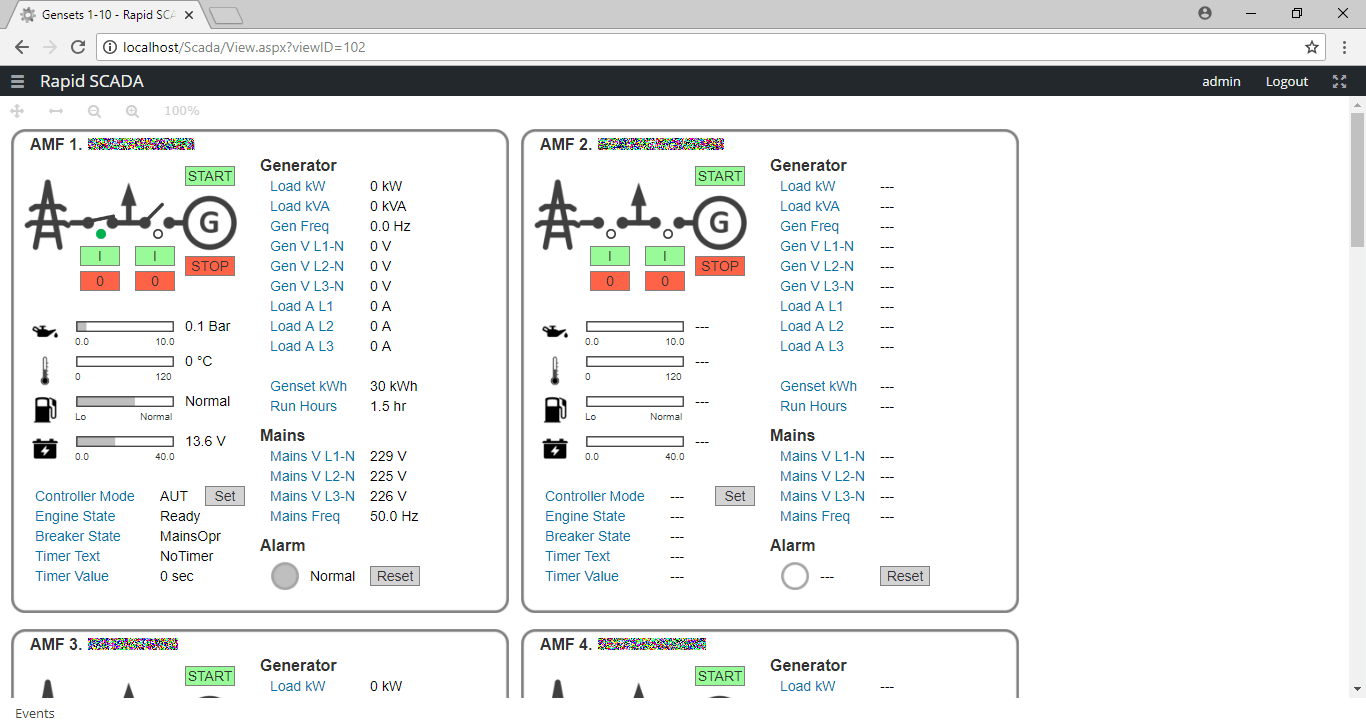
\includegraphics[width=15cm]{figuras/rapidscada.png}}
		}{
			\Fonte{\cite{RapidSCADA}.}
		}	
	    \end{figure}
	    
	    Outras informações importantes:
	    
	    \begin{alineascomponto}
	        \item É suportado por plataformas \textit{Windows} e \textit{Linux}.
    	    \item O sistema possui uma interface de administração no modelo cliente/servidor e outra de monitoramento no formato \gls{WEB}.
    	    \item Possui \textit{drivers} de comunicação, disponibilizados de forma gratuita, como: Modbus, \gls{OPC}, \gls{MQTT}, etc.
    	    \item Níveis de permissão de usuários, com controle de acesso.
    	    \item Alarmes de fogo e segurança, com avisos via interface.
    	    \item A empresa cobra por serviços de treinamento e suporte na ferramenta, além de comercializar módulos de software adicionais.
        \end{alineascomponto}
	    
    \section{Bancos de Dados}
    \label{sec:bancos-de-dados}
    
        \subsection{Relacionais}
        \label{sec:bancos-de-dados-relacionais}
            Oracle, MySQL, PostgreSQL
        
        \subsection{Não-Relacionais}
        \label{sec:bancos-de-dados-relacionais}
        \cite{cattell2011scalable}
        
            MongoDB, CouchDB e Cassandra